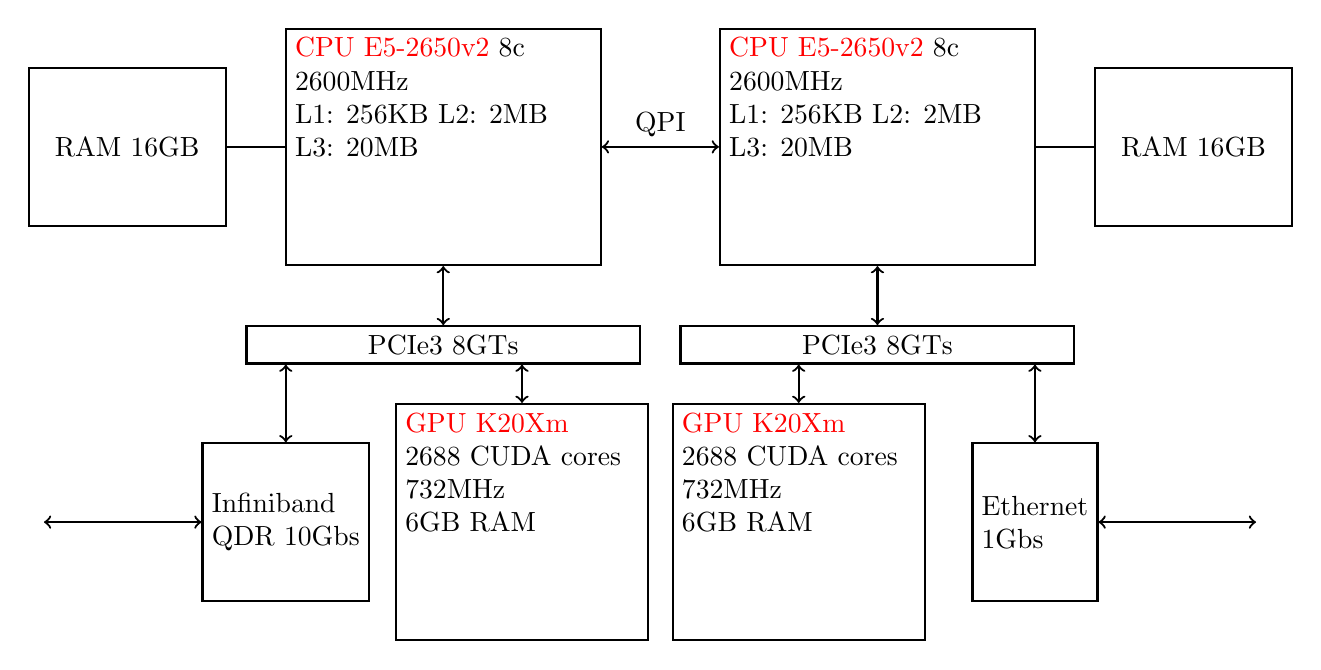
\begin{tikzpicture}[thick]
% CPUs
\node (CPU1) at (0,0) [draw,inner sep=0pt, minimum width=4cm, minimum height=3cm] {};
\node at (CPU1.north west) [below right, align=left]{{\color{red}{CPU E5-2650v2}} 8c\\2600MHz\\L1: 256KB L2: 2MB\\ L3:  20MB};
\node (CPU2) at ([xshift=3.5cm]CPU1.east) [draw,inner sep=0pt, minimum width=4cm, minimum height=3cm] {};
\node at (CPU2.north west) [below right, align=left]{{\color{red}{CPU E5-2650v2}} 8c\\ 2600MHz\\L1: 256KB L2: 2MB\\ L3:  20MB};
\draw[<->] (CPU1.east) -- (CPU2.west) node [above,midway] {QPI};

% RAM 
\node (RAM1) at ([xshift=-2cm]CPU1.west) [draw,inner sep=0pt, minimum width=2.5cm, minimum height=2cm] {RAM 16GB};
\node (RAM2) at ([xshift=2cm]CPU2.east) [draw,inner sep=0pt, minimum width=2.5cm, minimum height=2cm] {RAM 16GB};
\draw[-] (CPU1.west) -- (RAM1.east);
\draw[-] (CPU2.east) -- (RAM2.west);

% PCIe 
\node (PCIE1) at ([yshift=-1cm]CPU1.south) [draw,minimum width=5cm] {PCIe3 8GTs};
\node (PCIE2) at ([yshift=-1cm]CPU2.south) [draw,minimum width=5 cm] {PCIe3 8GTs};
\draw[<->] (PCIE1.north) -- (CPU1.south);
\draw[<->] (PCIE2.north) -- (CPU2.south);

% Networks 
\node (INFINIBAND) at ([yshift=-2cm,xshift=-2cm]PCIE1.south) [align=left,draw,minimum height=2cm] {Infiniband\\QDR 10Gbs};
\node (ETHERNET) at ([yshift=-2cm,xshift=2cm]PCIE2.south) [align=left,draw,minimum height=2cm] {Ethernet\\1Gbs};
\draw[<->] ([xshift=-2cm]PCIE1.south) -- (INFINIBAND.north);
\draw[<->] ([xshift=2cm]PCIE2.south) -- (ETHERNET.north);
\draw[<->] (INFINIBAND.west) -- ([xshift=-2cm]INFINIBAND.west);
\draw[<->] (ETHERNET.east) -- ([xshift=2cm]ETHERNET.east);

% GPUS
\node (GPU1) at ([yshift=-2cm,xshift=1cm]PCIE1.south) [align=left,draw,inner sep=0pt,minimum height=3cm, minimum width=3.2cm] {};
\node at (GPU1.north west) [below right, align=left] {{\color{red}{GPU K20Xm}}\\2688 CUDA cores\\732MHz\\6GB RAM};
\node (GPU2) at ([yshift=-2cm,xshift=-1cm]PCIE2.south) [align=left,draw,inner sep=0pt,minimum height=3cm, minimum width=3.2cm] {};
\node at (GPU2.north west) [below right, align=left] {{\color{red}{GPU K20Xm}}\\2688 CUDA cores\\732MHz\\6GB RAM};
\draw[<->] ([xshift=1cm]PCIE1.south) -- (GPU1.north);
\draw[<->] ([xshift=-1cm]PCIE2.south) -- (GPU2.north);
\end{tikzpicture}